\documentclass[11pt,a4paper]{article}
\usepackage[T1]{fontenc}
\usepackage[utf8]{inputenc}
\usepackage{amsmath,amssymb,amsthm,newtxtext,newtxmath,microtype}
\usepackage[margin=23mm,headheight=14pt,headsep=7mm,footskip=11mm]{geometry}
\usepackage{graphicx,booktabs,array,tabularx,enumitem,fancyhdr,caption,float,xcolor}
\usepackage[numbers,sort&compress]{natbib}
\usepackage[colorlinks=true,allcolors=blue!45!black,breaklinks=true]{hyperref}
\definecolor{ink}{HTML}{253640}\definecolor{accent}{HTML}{176B9B}
\pagestyle{fancy}\fancyhf{}\fancyhead[L]{\small Geometric root calculators}\fancyhead[R]{\small V21 / Research preprint}\fancyfoot[C]{\small\thepage}
\setlength{\parindent}{0pt}\setlength{\parskip}{5pt plus 1pt}\setlength{\emergencystretch}{3em}
\renewcommand{\arraystretch}{1.15}\captionsetup{font=small,labelfont=bf}
\setlist{noitemsep,topsep=3pt,leftmargin=*}\raggedbottom
\newtheorem{theorem}{Theorem}[section]\newtheorem{proposition}[theorem]{Proposition}
\newcommand{\map}[1]{\mathcal T_{\mathrm{#1}}}
\newcommand{\hub}[1]{\mathcal U_{#1}}
\newcommand{\fig}[3]{\begin{figure}[H]\centering\includegraphics[width=#2\linewidth]{figures/#1.pdf}\caption{#3}\end{figure}}
\hypersetup{pdftitle={Geometric Root Calculators: Fixed Circles, Moving Supports, and Analog Realization},pdfauthor={Ivan Besevic}}
\begin{document}\thispagestyle{empty}
{\small\sffamily\color{accent} CONSTRUCTIVE GEOMETRY / ITERATIVE COMPUTATION / ANALOG REALIZATION}\par
\vspace{8pt}
{\fontsize{24}{27}\selectfont\bfseries\color{ink} Geometric Root Calculators\par}
\vspace{5pt}{\large Fixed circles, moving supports, and analog realization}\par
\vspace{9pt}Ivan Besevic\footnote{Computational assistance: AI was used for derivations, proof development, figures and manuscript preparation. The author is responsible for the claims and their attribution. Section~\ref{sec:scope} distinguishes exact proofs, numerical checks and exploratory displays.}\quad$\cdot$\quad Independent research\par
{\small Version 21\quad$\cdot$\quad19 September 2026}\par
\url{https://github.com/ivan-fr/pandrosion}
\vspace{8pt}\hrule\vspace{8pt}
\textbf{Abstract.}
An iteration formula does not specify how to construct its next value. We study this realization problem for positive roots: encode the current estimate as a point, produce the residual by line intersections, and implement the correction with a geometric device. The central construction uses one prepared circle as a quadratic solver. It realizes an inverse Pad\'e correction of order five in $2p+2$ mobile joins, with an explicit rational preparation for every integer $p\ge3$. A second construction moves the radius of a decentered arc; it raises AD from order three to order five with the same mobile support operations and converges monotonically from every positive start. Fixed, moving and projective supports place these designs beside Newton, Halley and rational Pad\'e baselines. A binary geometric power module then connects the construction language to a centered, sampled analog implementation of the order-three AD map. We give the incidence arguments, convergence proofs, protocol counts and a concise map of the algebraic formalization. The analog application is supported by reproducible behavioral simulations; its device-level design remains a separate engineering task.

\section{Why construct an iteration?}
A numerical algorithm names operations. A physical calculator must realize them: a ratio may be an alignment, a product a similar-triangle construction, and a square root a circle crossing. Two formulas with the same local order can therefore have different realization costs. This paper asks which geometric arrangements make a root iteration economical and how that arrangement can guide an analog implementation.

The intended setting is constructive computation: exact incidence geometry supplies a design and a correctness argument; a count of mobile operations describes the protocol. It also exposes which quantities must be stored, copied or solved for in a circuit. Drawing cost and electrical delay are different quantities, but the decomposition into reusable operations connects them.

Our principal example is a fixed circle that solves for a correction rather than merely transferring a length. Three joins after the power stage complete a fifth-order update. The decentered-arc construction gives a complementary choice: global monotone convergence with a moving radius. The contribution is these explicit realizations and their analysis, rather than the classical Newton, Halley or Pad\'e families. Section~\ref{sec:scope} collects the proof and implementation boundaries; the main text develops the constructions themselves.
\clearpage

\section{Coordinates as reusable computing elements}\label{sec:rails}
Let $X>0$, let $p\ge3$ be an integer, and write
\[
 a=X^{-1/p},\qquad t=Xs^p,\qquad s^+=s\Phi(t),\qquad s>0.
\]
The state approaches the reciprocal root $a$; inversion supplies the desired $X^{1/p}$. We use $e=\log(s/a)$ for local error. Points are capital letters, scalar iteration maps are $\map{label}$, and polynomial coefficients use Greek letters. Thus a point and a correction function never share the same symbol.

In a rectangle with vertices $C=(0,0)$, $B=(W,0)$, $O=(0,H)$ and $A=(W,H)$, define two extended rails and a family of top centers:
\begin{equation}\label{eq:rails}
 R(q)=(W,H(1-q)),\quad L(q)=(0,H(1-q)),\quad
 \hub{f}=\left(\frac{Wf}{f-1},H\right).
\end{equation}
A line through the prepared center performs multiplication in one direction and division in the other:
\begin{equation}\label{eq:railops}
 \hub{f}R(q)\cap OC=L(fq),\qquad
 \hub{f}L(b)\cap AB=R(b/f).
\end{equation}
For example, substituting the first two points into a line equation and setting $x=0$ gives ordinate $H(1-fq)$. This is the whole arithmetic content of the rail device.

\subsection{The power stage}
Start at $P=R(s)$. The join $CP$ meets the top line at $V=\hub{1/s}$. A leftward projection through $\hub{1/2}$ followed by a return through $V$ changes a rail value $q$ to $sq/2$. After $p-1$ pairs, the endpoint is $Q=R(s^p/2^{p-1})$. Including the initial join, the stage uses $2p-1$ lines. Its normalization factor is part of the design, not discarded arithmetic.

More generally, choosing the leftward factors $f_1,\ldots,f_{p-1}$ gives an endpoint with value $s^p\prod_i f_i$. This allows the power stage to feed a device with its preferred residual scale. We use exactly this freedom for the fixed-circle calculator.

\subsection{A precise notion of work}
We count a join as $J$, a parallel-construction macro as $P_{\parallel}$, and a mobile compass arc as $C_{\mathrm{arc}}$. Intersections of already drawn objects, fixed preparation and final inversion are excluded. When expanded into ruler-and-compass traces, our parallel macro costs $2J+3C_{\mathrm{arc}}$. These conventions are specified before any cost comparison.

This question belongs to the constructive tradition of Lemoine's geom\'etrographie and d'Ocagne's nomography \cite{lemoine1902,docagne1925}. The Poncelet--Steiner theorem supplies a broad existence result for straightedge constructions with a given circle and its center \cite{steiner1833}. Our question is more specific: an explicit repeated protocol, its branch selection, and its mobile cost. The rectangle follows a modern Pandrosion reconstruction \cite{launayPandrosion}; historical interpretations are discussed in the archival V20 manuscript.
\clearpage

\section{A prepared circle as a quadratic solver}\label{sec:circle}
Suppose the desired correction factor is $v\approx1$. Instead of evaluating a rational approximation to $t^{-1/p}$, approximate the inverse relation $t=v^{-p}$ by a quadratic rational model and solve it exactly. Put
\begin{align}
 \alpha_p&=(p+1)(p+2),&\beta_p&=p^2-4,&\gamma_p&=(p-1)(p-2),\nonumber\\
 N(v)&=\gamma_pv^2-2\beta_pv+\alpha_p,&
 D(v)&=\alpha_pv^2-2\beta_pv+\gamma_p.\label{eq:model}
\end{align}
The model is $\mathcal R(v)=N(v)/D(v)$, the $[2/2]$ Pad\'e approximant of $v^{-p}$ at one. Its inverse branch $v(1)=1$ defines $\map{circle}(s)=sv(Xs^p)$. A circle can supply the quadratic root in a single crossing.

\subsection{The eight-line cubic example}
Use $W=2$, $H=4$, $p=3$ and $X=2$. Prepare a circle through $B$ with center $O_\Gamma$, a projector $Z$, and constants
\[
 O_\Gamma=(-152/113,126/113),\quad Z=(478/113,396/113),
 \qquad \rho=\tfrac12,\quad k=\tfrac5{113}.
\]
The first five joins form the rail power stage with left factors $\rho$ and $\sigma=20/113$, retaining $L_1=L(\rho s)$ and ending at $T=R(kXs^3)$. The last three joins are the main device:
\begin{enumerate}
\item Draw $ZT$ and select its prescribed intersection $G$ with the fixed circle.
\item Draw $BG$ to the top line, obtaining $U=\hub{\rho/v}$.
\item Draw $UL_1$ back to the right rail. Its value is $(\rho s)/(\rho/v)=sv$.
\end{enumerate}
\fig{fixed_circle}{1}{The fixed-circle device at $s=3/4$. Left: the sixth join supplies $G$, and the seventh supplies the readout center $U$. Right: an independently enlarged view shows the eighth join and distinguishes $P$ from $P^+$. The circle is drawn once, before iteration. Equal horizontal and vertical scales are used within each view.}
The computed next state is $0.793700551706633\ldots$, with relative error about $3.24\times10^{-8}$. The circle is doing arithmetic: it replaces a longer rational readout by the solution of a quadratic model.
\clearpage

\subsection{Why the inverse correction has order five}
The local order follows from one polynomial identity, which is also a useful certificate for the approximation. At $v=1$, $N=D=12$, and
\begin{equation}\label{eq:cert}
 pND+v(N'D-ND')=p\alpha_p\gamma_p(v-1)^4.
\end{equation}
Moreover $\gamma_pN=(\gamma_pv-\beta_p)^2+3(p^2-4)$ and $\alpha_pD=(\alpha_pv-\beta_p)^2+3(p^2-4)$, so the logarithms used below are well defined for $p>2$.

\begin{theorem}[Local inverse-circle order]
For real $p>2$, the inverse branch through $v=1$ exists near $t=1$ and satisfies
\begin{equation}\label{eq:circleorder}
 e^+=-\frac{(p^2-1)(p^2-4)}{720}e^5+O(e^7).
\end{equation}
It therefore alternates sides locally and has exact order five.
\end{theorem}
\begin{proof}
Set $v=1+u$, $E(u)=\log\mathcal R(1+u)/p$ and $K(u)=E(u)+\log(1+u)$. Equation~\eqref{eq:cert} gives
\[
 K'(u)=\frac{\alpha_p\gamma_pu^4}{(1+u)N(1+u)D(1+u)}.
\]
Thus $K(u)/u^5\to\alpha_p\gamma_p/720$, while $E(0)=0$ and $E'(0)=-1$. The inverse function theorem identifies $E(u)$ with the input logarithmic error. Dividing the limits gives the coefficient in~\eqref{eq:circleorder}. Analyticity and $\mathcal R(1/v)=1/\mathcal R(v)$ make the logarithmic update odd, giving the stated remainder. The coefficient is nonzero for $p>2$.
\end{proof}
The same identity, integrated as the derivative of $\log(v^p\mathcal R(v))$, proves the fifth-order Pad\'e contact. Model-based iteration and quadratic approximants have classical precedents \cite{traub1961,traub1964,shafer1974}; the construction problem is to realize this inverse with a short, prepared geometric device.

\subsection{Which circle intersection?}
The discriminant after removing a factor four is
\[
 \Delta_p(t)=(42p^2-24)t-3(p^2-4)(1+t^2).
\]
The transverse real interval is $\tau_-<t<\tau_+$, where
\[
 \tau_\pm=\frac{7p^2-4\pm4p\sqrt{3(p^2-1)}}{p^2-4},\qquad \tau_-\tau_+=1.
\]
Select the descending branch $\mathcal R'(v)<0$, equivalently
\[
 v_-<v<v_+,\qquad v_\pm=\frac{p^2+2\pm\sqrt{12(p^2-1)}}{p^2-4}.
\]
Its reference point is $v=1$. At $p=3,t=0.05$, both inverse roots are positive, approximately 3.1183 and 6.3817; only the first is on this branch. Positivity alone cannot choose $G$. At a transverse endpoint the two roots merge. Whole-interval contraction remains an explicitly separate conjecture in the archived study; the theorem above is local.
\clearpage

\subsection{The general-degree construction}\label{sec:generalcircle}
For each integer $p\ge3$, prepare $O_\Gamma=(h,j)$, $Z=(z_x,z_y)$, $k>0$ and $\rho>0$, using the rational formulas in Appendix~\ref{app:prep}. The circle passes through $B=(2,0)$ and is independent of $X$ and $s$. Put $\sigma=kX2^{p-3}/\rho$. The rail sequence uses
\[
 f_1=\rho,\quad f_i=\tfrac12\ (2\le i\le p-2),\quad f_{p-1}=\sigma.
\]
It saves $L_1=L(\rho s)$ and ends at $T=R(kt)$, because $\prod_i f_i=kX$. The same three final joins then give $R(sv)$.

\begin{theorem}[Counted finite-circle protocol]\label{thm:construction}
For the preparation in Appendix~\ref{app:prep}, assume $X,s>0$, $\tau_-<Xs^p<\tau_+$, and
\[
 s\ne1,\quad \sigma\ne1,\quad v\ne\rho,\quad
 b(v)=(2-h)2v-4j(\rho-v)\ne0.
\]
The selected branch is realized by $2p+2$ mobile joins using the prepared circle.
\end{theorem}
\begin{proof}
The power stage costs $1+2(p-1)=2p-1$ joins. To certify the remaining incidence, write
\[
 d=(2v,4(\rho-v)),\quad n=d\cdot d,\quad b=(B-O_\Gamma)\cdot d,
 \quad G=B-\frac{2b}{n}d.
\]
Then $G$ lies on the circle through $B$ and on the pencil line through $B$ and $\hub{\rho/v}$. Clearing $n$ in the collinearity condition for $Z,T,G$ gives
\begin{align*}
 I={}&(2-z_x)(-2bd_y-z_yn)\\
 &-[4(1-kt)-z_y][(2-z_x)n-2bd_x].
\end{align*}
The prepared parameters satisfy $I=\lambda_p[N(v)-tD(v)]$, with $\lambda_p\ne0$. Thus the selected inverse root places $G$ on $ZT$. Projecting $G$ through $B$, then $L_1$ through the resulting center, gives $R(sv)$ by~\eqref{eq:railops}. These are three joins. The branch arc is parameterized by $v_-<v<v_+$ and can be marked during preparation using its endpoints and $G(1)$. The listed hypotheses exclude an infinite center, a coincident $B,G$, and tangency; the other rail intersections are transverse.
\end{proof}
The exclusions concern this finite chart. In particular, $s=1$ sends the initial center $V$ to infinity even though the scalar correction can remain regular. A positive rescaling $\widetilde X=c^pX$, $\widetilde s=s/c$ preserves $t$ and conjugates every correction. A dyadic choice can keep the limiting state away from one, controlling the distant initial center near convergence. The circle-specific exclusions still require their own branch and chart checks.

The result is a concrete upper bound on mobile work, not merely an existence theorem for straightedge construction. Its advantage over the rational fifth-order baseline will be quantified after the other devices have been introduced.
\clearpage

\section{The five Pandrosion constructions}\label{sec:supports}
The fixed circle solves for a correction externally. A second architecture keeps the power endpoint $E=R(s^p)$ and changes the interception support inside the rectangle. Prepare $M=(0,H(1-X^{-1}))$. The slope of $ME$ is $m=H(1-t)/(WX)$. A line through $A$ of slope $k_s=H\kappa/(WX)$ meets the parallel to $ME$ through $P=R(s)$ at $T_A$. The horizontal through $T_A$ gives $P^+$, with
\begin{equation}\label{eq:common}
 s^+=s\frac{k_s}{k_s-m}=s\frac{\kappa}{\kappa-1+t}.
\end{equation}
This one identity explains the four accelerated supports; each is a different device for supplying $\kappa$. Their original power stage is the triangle chain: horizontals meet the diagonal $OB$ at $B_j=(Ws^j,H(1-s^j))$ and the left rail at $L_j=L(s^j)$. Parallels to $L_1B$ carry $B_j$ to $L_{j+1}$, by similar triangles. The $p$th horizontal gives $E=R(s^p)$.

\subsection{The original linear support MA}
We retain the original name MA, writing its lower-right endpoint as $A_{\rm lin}=B$ to keep the rectangle labels consistent. Intersect the parallel to $ME$ through $P$ with $MA_{\rm lin}=MB$, then take the horizontal readout. For $s\ne1$, the intersections give
\[
 \map{MA}(s)=1-\frac{X-1}{X S_p(s)},\qquad S_p(s)=\sum_{j=0}^{p-1}s^j.
\]
For $X>1$ this scalar map is increasing and $\map{MA}(s)-s=(1-Xs^p)/(XS_p(s))$. It therefore converges monotonically to $a$ from every positive start, with the removable scalar extension at $s=1$. Its derivative at $a$ is $1-pa^{p-1}/S_p(a)\in(0,1)$: convergence is linear.
\fig{pandrosion_ma}{.46}{Pandrosion MA, the linear reference construction, at $p=3,X=2,s=3/4$. Thin lines construct the power by similar triangles. The green parallel meets the blue support $MA_{\rm lin}$; the horizontal gives $P^+$. The historical endpoint $A_{\rm lin}$ is the lower-right vertex $B$ in this paper. At $s=1$ the unmodified geometric intersection is coincident, despite the removable scalar extension.}
\clearpage
\subsection{AK and centered AD: orders two and three}

\textbf{AK: a fixed line.} Prepare $K=(W(1-X/p),0)$. The support $AK$ has $\kappa=p$, so $\map{AK}(s)=ps/(p-1+t)$, Newton under inversion. It has order two and converges from every positive start.

\textbf{AD: a centered length transfer.} Prepare
\[
 O_{\mathrm{AD}}=\left(W-\frac{2W}{p-1},\ H-\frac{H(p+1)}{X(p-1)}\right).
\]
Transfer $AE=Hs^p$ downward from this center to $D_{\mathrm{AD}}$ and join $AD_{\mathrm{AD}}$. Then $\kappa=[p+1+(p-1)t]/2$, giving
\begin{equation}\label{eq:halley}
 \map{AD}(s)=s\frac{p+1+(p-1)t}{p-1+(p+1)t}.
\end{equation}
This is Halley, with cubic local order and global monotone positive convergence. Geometric interpretations of Halley precede this construction \cite{gander1985,scavo1995}; the support here is specified to preserve the common rail encoding and readout.

\begin{figure}[H]\centering
\begin{minipage}[t]{.48\linewidth}\centering
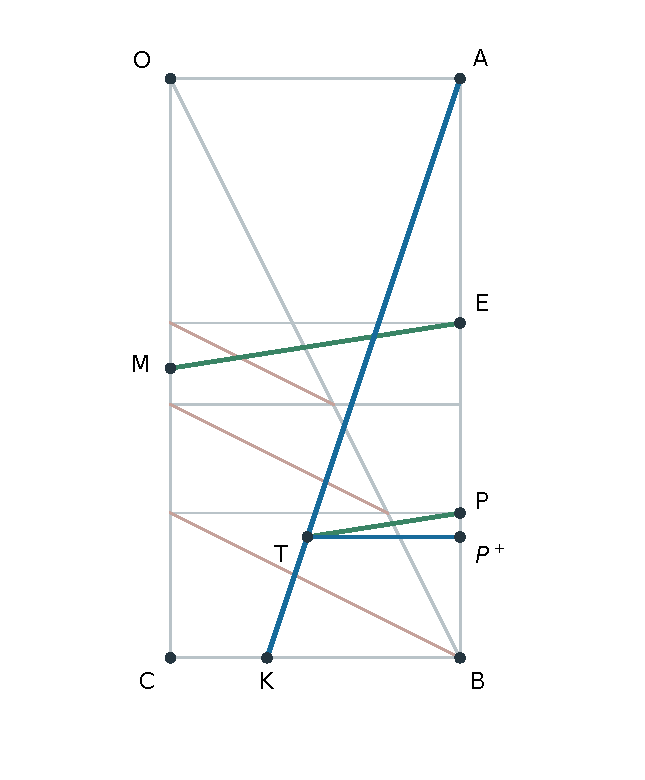
\includegraphics[width=\linewidth]{figures/pandrosion_ak.pdf}
\caption{Pandrosion AK, order two. The fixed support $AK$ replaces MA while the triangle chain and green correction direction are retained. Here $p=3,X=2,s=3/4$.}
\end{minipage}\hfill
\begin{minipage}[t]{.48\linewidth}\centering
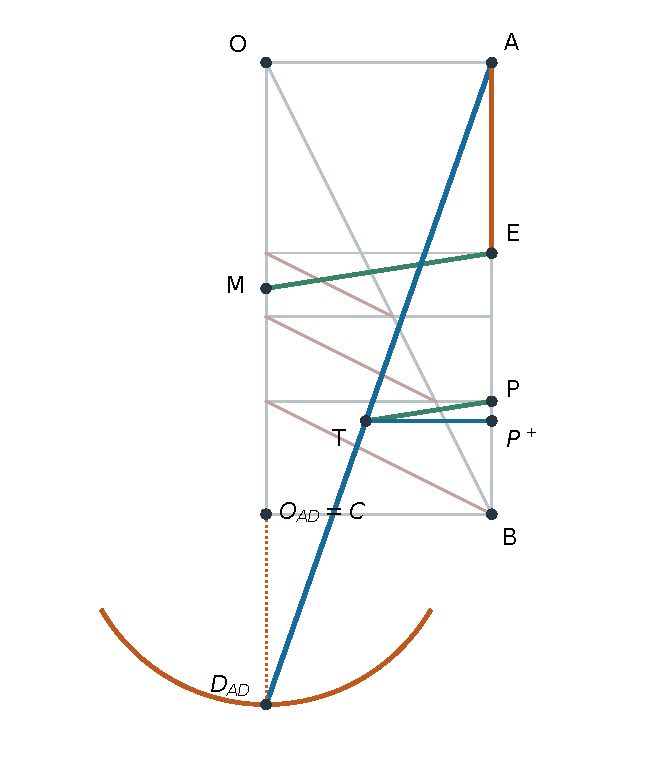
\includegraphics[width=\linewidth]{figures/pandrosion_ad.pdf}
\caption{Pandrosion AD, order three. Transfer the orange length $AE$ onto the prepared vertical through $O_{\rm AD}$; the lower arc point determines $AD_{\rm AD}$. Here $O_{\rm AD}=C$.}
\end{minipage}
\end{figure}
Both drawings preserve the full triangular power stage. The support encodes the correction law: a fixed slope for AK, or a radius-dependent slope for AD. The green transport and horizontal readout are otherwise identical.
\clearpage
\subsection{Projective AD: order four}
\textbf{Two joins supply the support.} Prepare
\[
 \ell:\ y=H\left(1+\frac{5p-1}{(p+1)X}\right),\quad
 Z_{\mathrm{proj}}=\left(W\left(1+\frac{5p-1}{2p(2p-1)}\right),H\left(1+\frac{p+1}{(2p-1)X}\right)\right).
\]
Set $D_{\mathrm{proj}}=Z_{\mathrm{proj}}E\cap\ell$ and join $AD_{\mathrm{proj}}$. Substitution in~\eqref{eq:common} gives
\begin{equation}\label{eq:proj}
 \map{proj}(s)=s\frac{2p((2p-1)t+p+1)}{(p+1)t^2+2(2p-1)(p+1)t+(2p-1)(p-1)}.
\end{equation}
The direct-root correction is Pad\'e $[2/1]$; the reciprocal-state factor displayed here is $[1/2]$. Denote its positive denominator by $Q_{\mathrm{proj}}(t)$. Direct differentiation gives
\[
 \map{proj}'(s)=-\frac{2p(p^2-1)(2p-1)(t-1)^3}{Q_{\mathrm{proj}}(t)^2}.
\]
The map has its global maximum $a$ at $s=a$. Also $\map{proj}(s)/s-1=(1-t)((p+1)t+5p-1)/Q_{\mathrm{proj}}(t)$. Thus a first step lands at or below $a$, and subsequent steps increase to $a$. Integrating the derivative at $a$ gives exact order four. The archival companion gives further dynamics and the original triangle-chain realization \cite{geometryv20}.

\fig{pandrosion_projective}{.49}{Projective AD [2/1], order four, at the same cubic state. The orange line $Z_{\rm proj}E$ meets the prepared horizontal $\ell$ at $D_{\rm proj}$. The blue support $AD_{\rm proj}$ receives the green correction. The inset separates $P$, $T$ and $P^+$.}
\textbf{The fifth construction.} Displacing the arc center from the prepared vertical makes the height a genuine square root. The decentered AD support is developed next, because its global fifth-order behavior changes the choice of device rather than only its coefficients.
\clearpage

\subsection{A decentered arc with a global fifth-order map}
For $p>2$, define
\begin{equation}\label{eq:arc}
 q(t)=\sqrt{\frac{(p-2)(t^2+1)+(10p+4)t}{12p}},\quad g(t)=(p-1)q(t),\quad
 \map{arc}(s)=s\frac{1+g(t)}{t+g(t)}.
\end{equation}
For integer $p\ge3$, put $\eta=(p-1)\sqrt{(p-2)/(12p)}$, $\zeta=(5p+2)/(p-2)$, $d_0=W/\eta$ and $\delta=(H/X)\sqrt{\zeta^2-1}$. Prepare
\[
 G_0=(W,H+H\zeta/X),\quad
 O_{\mathrm{arc}}=(W-d_0+\delta,H-H/(X\eta)),\quad x=W-d_0.
\]
Draw the arc centered at $O_{\mathrm{arc}}$ with radius $EG_0=(H/X)(t+\zeta)$ and take the lower intersection $D_{\mathrm{arc}}$ with the prepared vertical. Its vertical distance below the center is
\[
 \sqrt{EG_0^2-\delta^2}=\frac HX\sqrt{t^2+2\zeta t+1}.
\]
The support $AD_{\mathrm{arc}}$ consequently gives $\kappa=1+g(t)$ in~\eqref{eq:common}. All preparation parameters use rational operations and square roots of positive quantities. The radicand stays positive for $t>0$.
\fig{decentered_arc}{1}{The decentered-arc device for $p=7,X=W=2,H=4,s=3/4$. The full circle geometry is shown separately from the local report, at independently chosen equal-axis scales. The displacement $\delta$ makes the vertical circle intersection perform a square root. The local panel retains the complete support and distinguishes the reported state.}
Unlike the inverse-circle correction, this map is defined for every positive residual and requires no choice between two inverse-model branches. It uses a mobile radius at every step. Unlike rational diagonal Pad\'e, it realizes the correction with a single radical rather than two rational factors. These are practical differences in geometric realization, even though all three maps have fifth local order.

Centered AD and decentered AD use the same mobile support operations: one arc and one join. Their fixed preparations and coordinate scales differ. This is the precise sense in which order five is obtained at the mobile support cost of order three.
\clearpage

\subsection{Global monotone convergence of the decentered map}
\begin{theorem}\label{thm:arc}
For real $p>2$, $X>0$ and every $s_0>0$, \eqref{eq:arc} converges to $a$ monotonically without crossing it. Its logarithmic error satisfies
\begin{equation}\label{eq:arcorder}
 e^+=\frac{(p-2)(p^2-1)(3p+1)}{1440}e^5+O(e^7).
\end{equation}
\end{theorem}
\begin{proof}
The radicand is positive and $q(1/t)=q(t)/t$, so the correction is reciprocal. Write
\[
 \mathcal E(t)=\frac{\log t}{p}+\log(1+g(t))-\log(t+g(t)).
\]
Define the auxiliary polynomials
\begin{align*}
 A_*(t)&=(p-1)(t^2+1)+(10p+2)t,\\
 B_*(t)&=(t+1)(6pt-(t-1)^2),\\
 K_*(t)&=(p^2-5p-2)(t-1)^2+12p(3p+1)t.
\end{align*}
Differentiation and factorization give
\begin{align}
 \frac{d\mathcal E}{d\log t}
 &=\frac{(p-2)(p-1)^2(qA_*-B_*)}{12p^2g(1+g)(t+g)},\label{eq:arcder}\\
 q^2A_*^2-B_*^2&=\frac{p+1}{12p}(t-1)^4K_* .\label{eq:arcfactor}
\end{align}
Here $A_*>0$. If $B_*\le0$, then $qA_*-B_*>0$. Otherwise $(t-1)^2<6pt$. When $p^2-5p-2\ge0$, $K_*>0$ directly; otherwise
\[
 K_*=6p^2(p+1)t+(p^2-5p-2)((t-1)^2-6pt)>0.
\]
Equation~\eqref{eq:arcfactor} now gives $qA_*>B_*$ for $t\ne1$. Therefore $\mathcal E$ is strictly increasing with $\mathcal E(1)=0$: the new logarithmic error has the old sign. Meanwhile $\Phi(t)-1=(1-t)/(t+g)$ moves the state toward the root. The orbit is monotone and bounded between $s_0$ and $a$. Its positive limit is a fixed point by continuity, and $\Phi(t)=1$ implies $t=1$.

Near one, rationalize $qA_*-B_*$ using~\eqref{eq:arcfactor}. Since $q=1$, $g=p-1$, $A_*=B_*=12p$ and $K_*=12p(3p+1)$ at $t=1$, this gives
\[
 \lim_{t\to1}\frac{d\mathcal E/d\log t}{(t-1)^4}
 =\frac{(p-2)(p^2-1)(3p+1)}{288p^5}.
\]
Substituting $t=e^{pe}$ and integrating yields~\eqref{eq:arcorder}; reciprocity makes the analytic logarithmic map odd.
\end{proof}
At $p=3$, the leading coefficient is $+1/18$, whereas the fixed-circle inverse has $-1/18$. The former stays on the starting side; the latter alternates near the root. At $p=2$, both scalar radical formulas reduce to the exact square-root correction, but the displayed decentered preparation must be replaced by a mean-proportional construction.
\clearpage

\section{What the shorter construction saves}\label{sec:cost}
A useful comparison holds the state, requested accuracy and counting convention fixed. The rational competitors can be built on the same rail telescope. A prepared projector
\[
 Z(\mu,\nu)=\left(-\frac{W\mu}{1-\mu},H\left(1-\frac{\nu}{1-\mu}\right)\right)
\]
sends $Q=R(q_p)$ to $\hub{f(q_p)}$, with $f(q)=\mu+\nu/q$. Two such projections and two rail joins multiply a stored value by $f/g$: a four-join module.

For Halley choose $f=(p-1)/(4p)+(p+1)/(4pt)$ and $g=(p+1)/(4p)+(p-1)/(4pt)$. Since $t=X2^{p-1}q_p$, each is of the required projector form. The cost is $2p-1+4=2p+3$ joins.

For rational diagonal Pad\'e set $a_5=(p-1)(2p-1)$, $b_5=8p^2-2$, $c_5=(p+1)(2p+1)$. The correction is
\[
 \Phi_{\mathrm{rat}}(t)=\frac{a_5t^2+b_5t+c_5}{c_5t^2+b_5t+a_5}
 =\prod_{r\in\{r_+,r_-\}}\frac{t+r}{rt+1},\quad
 r_\pm=\frac{b_5\pm\sqrt{12p^2(4p^2-1)}}{2a_5}.
\]
Each factor uses the four-join module with $f_r=[1+r/t]/[2(1+r)]$ and $g_r=[r+1/t]/[2(1+r)]$. Both reuse $Q$, giving $2p+7$ joins. Its scalar map is globally monotone: its derivative is $a_5c_5(t-1)^4/(c_5t^2+b_5t+a_5)^2$, and numerator minus denominator is $6p(1-t)(1+t)$.

\begin{table}[H]\centering\small
\caption{Generic mobile protocol costs; fixed preparation and final inversion are excluded. A parallel macro is $2J+3C_{\mathrm{arc}}$. The scope column describes the exact scalar map.}
\begin{tabularx}{\linewidth}{@{}Xccccc@{}}\toprule
Construction & Order & $J$ & $P_{\parallel}$ & $C_{\mathrm{arc}}$ & Scope\\\midrule
MA rectangle & 1 & 2 & $2p+1$ & 0 & $X>1$\\
AK rectangle & 2 & 2 & $2p+1$ & 0 & Global\\
AD rectangle & 3 & 3 & $2p+1$ & 1 & Global\\
Projective AD & 4 & 4 & $2p+1$ & 0 & Global\\
Decentered AD & 5 & 3 & $2p+1$ & 1 & Global\\
Pencil Halley & 3 & $2p+3$ & 0 & 0 & Global\\
Pencil rational Pad\'e & 5 & $2p+7$ & 0 & 0 & Global\\
Fixed-circle inverse & 5 & $2p+2$ & 0 & 0 & Local\\\bottomrule
\end{tabularx}
\end{table}
The fixed circle saves five joins per update relative to the rational fifth-order realization. For $p=3,X=2,s_0=3/4$, reaching 60 reciprocal-state decimal digits takes four Halley steps (36 joins), three rational fifth-order steps (39 joins), or three fixed-circle steps (24 joins). The decentered map also takes three steps, using its different arc-and-parallel budget. These are construction-work comparisons; they do not predict circuit time or energy.

Rectangle counts use the original linear triangle power chain. After the first update, its final horizontal can be reused, saving one parallel. The binary power replacement below has its own count and must not be combined with $2p+2$ as though the protocols were identical.
\clearpage

\section{Binary geometry and the path to an analog calculator}\label{sec:binary}
The linear telescope is attractive for a few degrees. At large $p$, binary powering gives a smaller arithmetic architecture. Define a top encoding $Z_\times(q)=(W+Hq,H)$ and the fixed unit $U_\times=(W+H,H)$. A parallel to $U_\times B$ copies $R(a)$ to $Z_\times(a)$. The parallel through $Z_\times(a)$ to $U_\times R(b)$ then meets the right rail at $R(ab)$: its slope is $b$ and its horizontal displacement is $-Ha$.

Squaring the accumulator and multiplying by $s$ at each binary one produces $E=R(s^p)$. With $L=\lfloor\log_2p\rfloor$ and $h=\operatorname{popcount}(p)$, there are $m=L+h-1$ multiplications. Reusing the top copy of $s$, the power stage costs $mJ+(m+L)P_{\parallel}$. It feeds any of the four rectangle supports unchanged.
\fig{fast_geometry}{1}{The fast-power construction and its AD readout, adapted from the V30 companion. The case $p=13=(1101)_2$ uses five products along exponents $1,2,3,6,12,13$. A product is an actual pair of line incidences, not a numerically inserted power. The output $E$ enters the same moving support and horizontal readout.}
This is the bridge to analog design: multiplication cells can follow the same binary schedule, while memory retains the state between AD updates. The geometry identifies the arithmetic dependencies; an electrical representation must additionally control their sensitivity and settling behavior.
\clearpage

\subsection{A centered electrical representation}
Directly encoding a normalized state $u\approx1$ is poorly conditioned at large degree: for $t=Yu^p$, $\partial\log t/\partial u=p/u$. The prototype first prepares a digital scale $c$ with $Y\approx Xc^p\in[1,2]$, writes $s=cu$, and stores
\[
 q=p(u-1),\qquad d_n=\frac pn(u^n-1),\qquad \widehat r=\frac1{c(1+q/p)}.
\]
Then $\partial\log t/\partial q=1/u$. The geometric product schedule becomes the exact polynomial recurrence
\begin{align*}
 d_{2n}&=d_n+\frac n{2p}d_n^2,\\
 d_{n+1}&=d_n+\frac{q-d_n}{n+1}+\frac n{p(n+1)}d_nq,\\
 t&=Y(1+d_p),\qquad
 q^+=q+\frac{2(1+q/p)(1-t)}{1+t+(t-1)/p}.
\end{align*}
Thus the electrical system realizes order-three AD in different state coordinates. There are 25 power stages at $p=10^6$ and at most 37 over the programmed range $3\le p\le10^6$.

The V30 companion implementation \cite{analogv30} uses behavioral voltage sources for arithmetic, explicit RC loading, buffered storage and timed switches. Its precision mode adds electrical-reference calibration, leakage compensation, 100 nF memories and a calibrated 24-bit ADC transfer model. The following drawing makes the memory and loading assumptions visible, rather than treating a formula as a completed electronic circuit.
\fig{analog_circuit}{.84}{Electrical topology from the V30 behavioral prototype: candidate and next-state memory, explicit state disturbances and a loaded arithmetic cell. Diamonds represent behavioral voltage sources; the RC elements and switch connections are explicit in the netlist. The ADC is a separate transfer model. This realization concerns the AD map, not the fifth-order circle devices.}
\clearpage

\subsection{What the analog application establishes}
The generalist arithmetic campaign covers 8,243 input pairs and 4,278 degrees. A separate calibrated SPICE campaign meets one ppm relative decoded-root error on 64 validation cases, with largest error 0.279 ppm at a 23.985 ms scheduled readout. A faster fixed policy reads at 4.785 ms and stays below one ppm on 18 new cases; retrospective evaluation of the previous 64 trajectories reaches 0.982 ppm. These datasets answer different questions and are kept separate in the companion paper and repository.

The high-degree example also clarifies where the work is done. At $p=10^6,X=500000$, digital interval preparation already gives $1/c$ with relative error about $2.477\times10^{-7}$. The analog loop refines this estimate. Accordingly, a fair hardware comparison includes preparation, programming and conversion. The recorded circuit times exclude those costs; no advantage over optimized digital root calculation has been demonstrated.

The geometric contribution remains useful at this stage: it supplies exact computational primitives, alternative correction devices and a transparent route to a circuit architecture. It does not turn line counts into speed claims. The fixed-circle and decentered fifth-order designs are candidates for further electrical realization; the implemented companion studies order three.

\section{Evidence, scope and reproducibility}\label{sec:scope}
\textbf{Mathematical scope.} The written proofs establish the fixed-circle local fifth-order result and the decentered map's global monotone convergence. The linear MA argument follows directly from its increasing scalar map; the finite diagram excludes its coincident state. The rational baselines belong to classical iteration families \cite{dlmf38,laszkiewicz2009,baker1996}. The explicit arrangements and counted protocols are the objects proposed here; their historical priority and optimality remain open. Iterative approximation of a cube root is distinct from its exact finite straightedge-and-compass construction.

\textbf{Formal scope.} Lean and mathlib \cite{lean4,mathlib} serve as algebraic and incidence checks, with additional analytic theorems where the modules actually export them. It is not used as a blanket label for the entire paper. The relevant map is concise:
\begin{center}\small
\begin{tabularx}{\linewidth}{@{}p{.34\linewidth}X@{}}\toprule
Module family & What the checked development supplies\\\midrule
\texttt{RectangleProjective} & Projection/readout identities and order-four dynamics.\\
\texttt{RectanglePencils*} & Rail operations, rational projectors, dynamics and order results.\\
\texttt{RectangleFixedCircle} & Quadratic identities, radical charts, preparation certificates, readout and a parameterized local limit.\\
\texttt{RectangleDecenteredArc} & Polynomial certificates used in the written radical proof.\\
\texttt{RectangleFastPower} & Product incidence and geometric binary recursion.\\
\texttt{AnalogFastAD} & Six exact centered-arithmetic identities.\\\bottomrule
\end{tabularx}\end{center}
The full radical convergence argument, inverse-branch assembly and physical trace count are written arguments. Neither Lean nor the numerical checks certify the browser renderer, device noise, ADC implementation or fabricated silicon. The named audits restrict transitive axioms to the standard \texttt{propext}, \texttt{Classical.choice} and \texttt{Quot.sound}; a repository-wide module count is not a count of this paper's proved claims.

\subsection{A direct route through the repository}
Start with \texttt{paper/reciprocal\_geometry\_v21/README.md}. It links the article, its editable figures, a verification entry point and the precise proof modules. The geometry gallery at \url{https://ivan-fr.github.io/pandrosion/} lets the reader inspect each join and iterate the constructions. The spherical view is retained there as an interface feature; the mathematical constructions are planar.

The verification entry point reruns the archived revision, radical-arc and fixed-circle checks. These include symbolic identities, high-precision independent line/circle intersections and scalar comparisons. The original fixed-circle study tests 162 configurations at 250 digits; the arc study tests 108 at 160 digits. They supplement the written proofs and expose implementation mistakes. The frozen V20 and analog V30 packages remain accessible as detailed companions rather than prerequisites to finding the main result.

Citation metadata accompany this version. The paper source, editable figures and datasets are versioned, and the PDF is rebuilt by CI.

\section{Conclusion}
The main result is a geometric calculator: a rationally prepared circle converts a quadratic model into a fifth-order correction using three joins beyond a rail power stage. A second device, the decentered arc, offers global monotone convergence while preserving AD's mobile arc-and-join budget. These constructions make the difference between a numerical formula and its realization explicit.

The binary product gadget extends the same design language to large degrees. Its centered electrical translation has a reproducible behavioral implementation for AD, with measured simulation tradeoffs between precision and time. This gives the geometric program a concrete application while leaving the fifth-order electrical designs as a clearly identified next step.

The useful open questions are now specific: full-branch contraction of the inverse-circle map, better-conditioned finite charts, and an electrical implementation of the radical correction with a measured cost. Answering them would strengthen the connection between constructive geometry and physical computation.

\appendix
\section{Rational preparation for every integer degree}\label{app:prep}
This appendix makes the general-circle protocol reproducible without searching through an earlier manuscript. Write $\nu=p-3$ and use $\alpha_p,\gamma_p$ from~\eqref{eq:model}. Define
\begin{align*}
 \mathcal D_p&=625\nu^5+10525\nu^4+56797\nu^3+88639\nu^2+14758\nu+664,\\
 \mathcal K_p&=625\nu^5+1975\nu^4+4147\nu^3+2905\nu^2+448\nu+340,\\
 \chi_p&=288p(p-2)(25p^2-244)/\mathcal D_p,\\
 u_p&=5-4\alpha_p/(9\gamma_p),\qquad w_p=8(5-2p)/(9(p-1)).
\end{align*}
Take
\begin{align*}
 \rho&=\tfrac13,& k&=\mathcal K_p/\mathcal D_p,& j&=-3\chi_pw_p/4,\\
 h&=2+2j-\chi_pu_p/2,&z_x&=2-\chi_p,&
 z_y&=\frac{384p(25p^3-50p^2-415p+974)}{\mathcal D_p}.
\end{align*}
Then the incidence certificate in Theorem~\ref{thm:construction} has multiplier $\lambda_p=-64k\chi_p/(9\gamma_p)$. The positive coefficients imply $\mathcal D_p,\mathcal K_p>0$ for $\nu\ge0$; $25p^2\ne244$ for integer $p\ge3$ makes $\chi_p,\lambda_p,j$ nonzero. All parameters are rational. The circle is drawn with center $(h,j)$ through $B$. This uniform chart is checked symbolically; the Lean preparation certificates cover the compact chart below and the separate degree-four specialization.
At $p=4$ the formulas give the finite values
\[
 k=145/2389,\quad O_\Gamma=(13502/7167,3328/2389),\quad
 Z=(-214/2389,2432/2389).
\]
The cubic worked example uses a more compact chart. For $p\ne4$, put $\Lambda_p=p^3+12p^2+39p-26$ and take
\begin{align*}
 \rho&=\tfrac12,& k&=\frac{(p-2)(p^2-4p+13)}{\Lambda_p},\\
 h&=2-\frac{72p(p+4)}{(p-1)\Lambda_p},&
 j&=\frac{24p(p-2)(p+4)}{(p-1)\Lambda_p},\\
 z_x&=2-\frac{24p(p+4)(p-2)}{(p-4)\Lambda_p},&
 z_y&=\frac{24p(p^2+2p-26)}{(p-4)\Lambda_p}.
\end{align*}
Here $\lambda_p=-384p(p-2)(p+4)(p^2-4p+13)/[(p-4)(p-1)\Lambda_p^2]$. Substitution checks both charts. For numerical evaluation the branch can be written without the removable cancellation at large $t$:
\[
 v(t)=\begin{cases}
 \dfrac{\alpha_p-t\gamma_p}{\beta_p(1-t)+\sqrt{\Delta_p(t)}},&t\le1,\\[5pt]
 \dfrac{\sqrt{\Delta_p(t)}-\beta_p(1-t)}{t\alpha_p-\gamma_p},&t>1.
 \end{cases}
\]
\begingroup\small\setlength{\bibsep}{1pt}
\bibliographystyle{unsrtnat}\bibliography{references}\endgroup
\end{document}
